
\documentclass[11pt,a4paper]{article}
\usepackage[left=22mm,right=22mm,top=24mm,bottom=24mm]{geometry}
\usepackage{fontspec}
\setmainfont{Liberation Serif}
\usepackage{polyglossia}
\setdefaultlanguage{russian}
\setotherlanguage{english}
\usepackage{amsmath,amssymb,mathtools,bm}
\usepackage{booktabs,longtable,array,multirow}
\usepackage{graphicx}
\usepackage{caption}
\usepackage{subcaption}
\usepackage{tabularx,adjustbox,ragged2e,makecell}
\usepackage{xcolor}
\usepackage{hyperref}
\usepackage{pdflscape}
\hypersetup{colorlinks=true,linkcolor=blue,urlcolor=blue,citecolor=blue}
\usepackage{enumitem}
\setlist[itemize]{topsep=2pt,itemsep=2pt,leftmargin=1.4em}
\setlength{\parindent}{0pt}
\setlength{\parskip}{5pt}
\captionsetup{font=small}
\newenvironment{fittable}[1][\small]{%
  \par\medskip
  \begin{center}
  #1
  \setlength{\tabcolsep}{4.5pt}%
  \renewcommand{\arraystretch}{1.10}%
  \begin{adjustbox}{max width=\linewidth}
}{%
  \end{adjustbox}
  \end{center}
  \par\medskip
}

\title{Игрушечный пример управления 7-летним процентным свопом\\[2mm]
\large Сравнение пяти rate-risk метрик, пяти сценариев и пяти политик}
\author{Сгенерировано автоматически на базе Python / LaTeX}
\date{}

\begin{document}
\maketitle

\begin{center}
\fbox{\parbox{0.94\linewidth}{
\textbf{Что именно сделано.} Построен toy-example в духе \textit{control under constraints}: short rate следует one-factor Hull-White, инструмент --- 7Y payer swap, управление идет через скорость изменения номинала $u_t=\dot q_t$, а капитал $K_t$ несет: (i) coupon/carry по свопу, (ii) жесткий штраф за нарушение риск-аппетита $K_t/q_t < CAR$, (iii) квадратичный liquidity cost $\lambda \dot q_t^2/2$. Сравниваются пять метрик риска по ставке --- $\partial_r \Delta_{0.5y}K$, $\partial_r \Delta_{1y}K$, $\partial_r \Delta_{3y}K$, $\partial_r MtM$ и $\partial_r V$ --- на пяти сценариях и пяти политиках.
}}
\end{center}

\section*{1. Модель и toy-упрощения}
Рынок моделируется one-factor Hull-White / Ornstein-Uhlenbeck short-rate динамикой
\[
 dr_t = a(\bar r - r_t)dt + \sigma_t dW_t,
\]
где в базовой калибровке $a=0.35$, $\bar r=2.50\%$, $\sigma=1.20\%$. Для построения value surfaces мы используем одну и ту же динамику под real-world и pricing measure: это сознательное toy-упрощение, которое позволяет сконцентрироваться на сравнении метрик и политик, а не на калибровочных деталях.

Инструмент --- 7-летний payer swap с квартальным шагом и исходным номиналом $q_0=100$. В toy-оценке оставшегося свопа используется local-flat-curve proxy по текущей short rate $r_t$. Для оставшихся дат $T_i>t$ единичный MtM задается как
\[
 m_t(r) = 1 - e^{-r(T_N-t)} - K_{fix}\sum_{i:t<T_i\le T_N} \Delta t\, e^{-r(T_i-t)},
\]
а портфельный MtM равен $MtM_t = q_t m_t(r_t)$. Поэтому delta рынка для этой метрики равна
\[
 \partial_r MtM_t = q_t\Bigg[(T_N-t)e^{-r_t(T_N-t)} + K_{fix}\sum_{i:t<T_i\le T_N} \Delta t\,(T_i-t)e^{-r_t(T_i-t)}\Bigg].
\]

Капитал обновляется на дискретной квартальной сетке. В начале шага мы меняем номинал на $q_{t+} = q_t + u_t\Delta t$ и затем за шаг получаем
\[
 \Delta K_t = q_{t+}(r_t-K_{fix})\Delta t
 - \mathbf{1}\!\left(\frac{K_t}{q_{t+}}<CAR\right)\frac{\Delta t}{\varepsilon}
 - \frac{\lambda}{2}u_t^2\Delta t.
\]
Здесь $CAR=10\%$, $\varepsilon=0.25$, $\lambda=0.0020$. Для удобства оптимальный контроль ищется на дискретном множестве скоростей
\[
 u_t \in \{-40,-20,0,20,40\}.
\]

\begin{fittable}
\begin{tabular}{lll}
\toprule
Параметр & Значение & Комментарий \\
\midrule
$\Delta t$ & 0.25y & Quarterly control / coupon step \\
$T$ & 7y & Swap maturity \\
$a$ & 0.35 & Hull-White mean reversion \\
$\bar r$ & 2.50\% & Long-run short rate and initial flat curve level \\
$\sigma$ & 1.20\% & Baseline short-rate volatility \\
$K_{fix}$ & 2.508\% & Par fixed coupon at $t=0$ \\
$q_0$ & 100 & Initial swap notional \\
$K_0$ & 14.0 & Initial capital \\
$CAR$ & 10\% & Risk-appetite floor $K_t/q_t$ \\
$\varepsilon$ & 0.25 & Breach penalty $1/\varepsilon=4$ per year \\
$\lambda$ & 0.0020 & Liquidity cost coefficient \\
$u_t$ & $\{-40,-20,0,20,40\}$ & Optimal-control action set (notional units/year) \\
\bottomrule
\end{tabular}

\end{fittable}

\section*{2. Метрики риска и политики}
Для каждой фиксированной политики $\pi$ вычисляются три horizon-метрики накопленного капитала
\[
 \Delta_TK_t^\pi(s) = \mathbb{E}^{RW}\!\left[\sum_{j=t}^{t+T-\Delta t} \Delta K_j \mid s_t=s\right], \qquad T\in\{0.5y,1y,3y\},
\]
а также рыночный MtM и полная control-aware стоимость
\[
 V_t(s)=\sup_u\; \mathbb{E}\left[\sum_{j=t}^{T-\Delta t} e^{-r_j\Delta t}\Delta K_j\mid s_t=s\right], \qquad s=(r_t,q_t,K_t).
\]
Во всех случаях анализируется именно процентный риск через чувствительность по текущей ставке,
\[
 \mathcal{D}^M_t = \frac{\partial M_t}{\partial r_t}.
\]
На практике $\partial_r \Delta_TK$ и $\partial_r V$ получаются из value surfaces через центральную разность по оси $r$.

Сравниваемые политики.

\begin{fittable}
\begin{tabular}{lll}
\toprule
Политика & Правило & Интерпретация \\
\midrule
Passive q & $u_t=0$ & Пассивно держим исходный номинал. \\
CAR-target & $q^*=\min(q_{max},K_t/CAR)$ & Подтягиваем номинал к целевому капиталовому плечу. \\
MtM-band & $|q_t m_t(r_t)|\le M^*$, $M^*=3$ & Сжимаем позицию, когда абсолютный MtM уходит из полосы. \\
0.5y-greedy & $u_t=\arg\max \Delta_{0.5y}K_t$ & Рецедирующий горизонт: оптимизация только на полгода. \\
Optimal V & $u_t=\arg\max V_t$ & Полный Беллман на весь остаточный срок. \\
\bottomrule
\end{tabular}

\end{fittable}

\section*{3. Сценарии рынка}
Сценарии --- это не новая модель, а пять осмысленных pathwise реализаций той же Hull-White динамики. Они заданы через разные последовательности шоков $z_n$ и, в одном случае, через hump-shaped $\sigma_t$.
Все value surfaces для $\Delta_{0.5y}K$, $\Delta_{1y}K$, $\Delta_{3y}K$ и $V$ пересчитываются один раз под базовой калибровкой, а затем политики прогоняются на stress-paths ретроспективно. Это важно: сценарии здесь используются как ex-post тестирование правил управления, а не как отдельные калибровки модели.

\begin{fittable}
\begin{tabular}{ll}
\toprule
Сценарий & Конструкция \\
\midrule
Base MR & mean reversion with moderate shocks \\
Early sell-off & positive shocks over the first 18 months \\
Rally & negative shocks over the first 18 months \\
Hump vol & volatility hump around year 1.5 \\
Whipsaw & alternating shocks with slightly higher vol \\
\bottomrule
\end{tabular}

\end{fittable}

\begin{figure}[htbp]
  \centering
  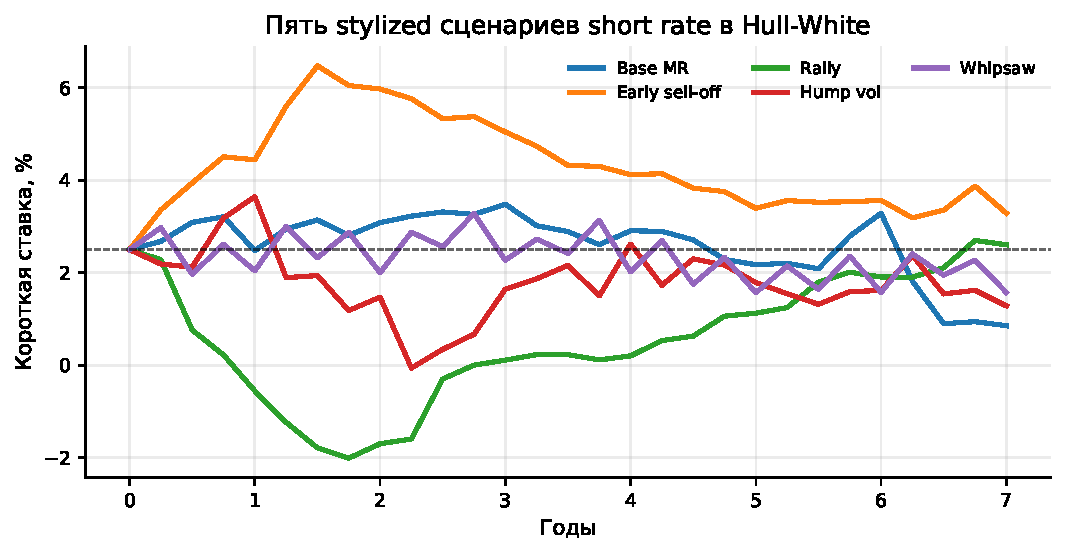
\includegraphics[width=0.96\linewidth]{figures/scenario_paths.pdf}
  \caption{Пять stylized сценариев short rate. Hump vol отличается именно выпуклой во времени волатильностью; остальные --- разными shock-patterns при постоянной базовой $\sigma$.}
\end{figure}

\section*{4. Ключевые результаты}
\subsection*{4.1. Что делают политики в stress-сценарии с hump-волатильностью}
\begin{figure}[htbp]
  \centering
  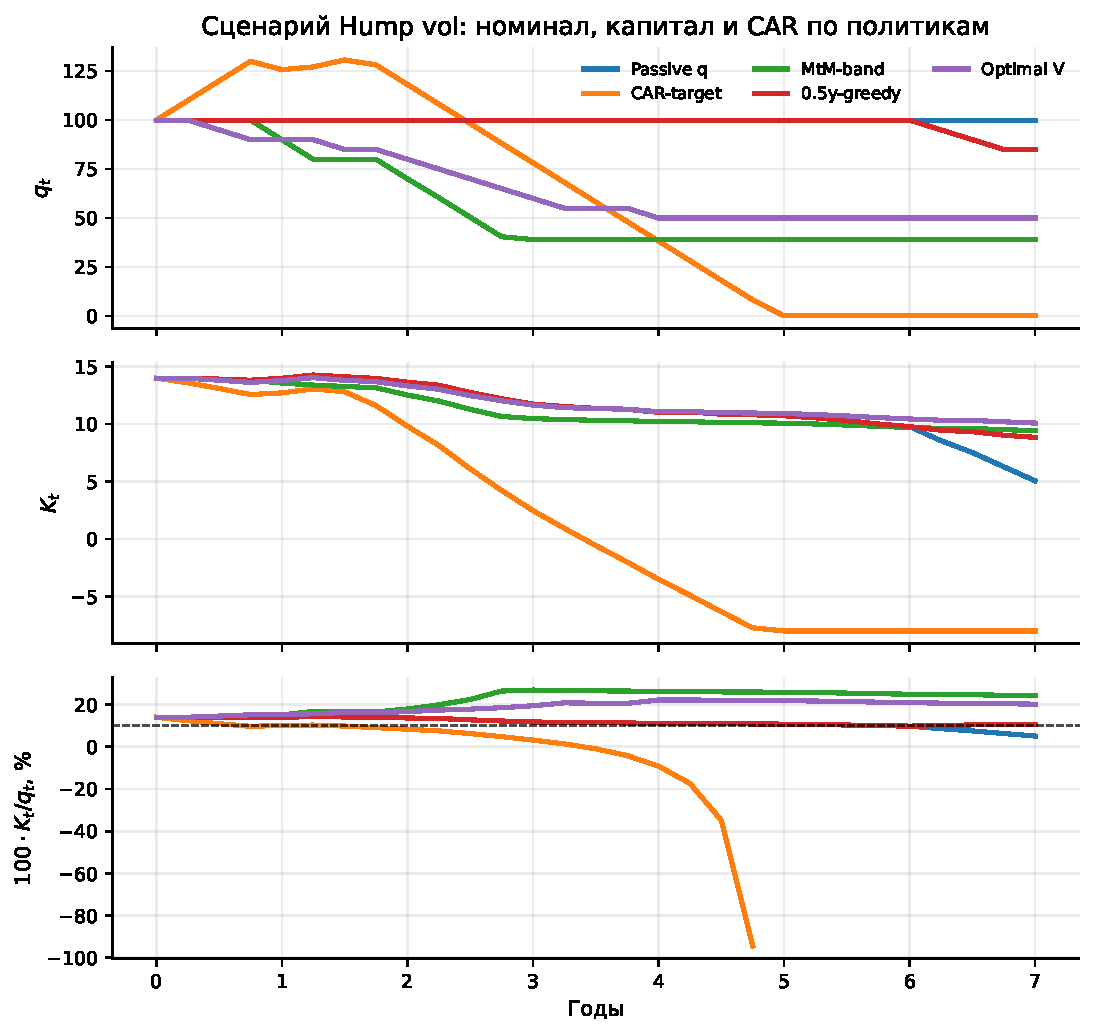
\includegraphics[width=0.96\linewidth]{figures/hump_policy_paths.pdf}
  \caption{Сценарий Hump vol. Пассивная позиция держит номинал и теряет капитал. MtM-band и full-optimal рано сжимают позицию; optimal делает это мягче, чем CAR-target, и потому сохраняет больше капитала.}
\end{figure}

\subsection*{4.2. Как ведут себя пять deltas у оптимальной политики}
\begin{figure}[htbp]
  \centering
  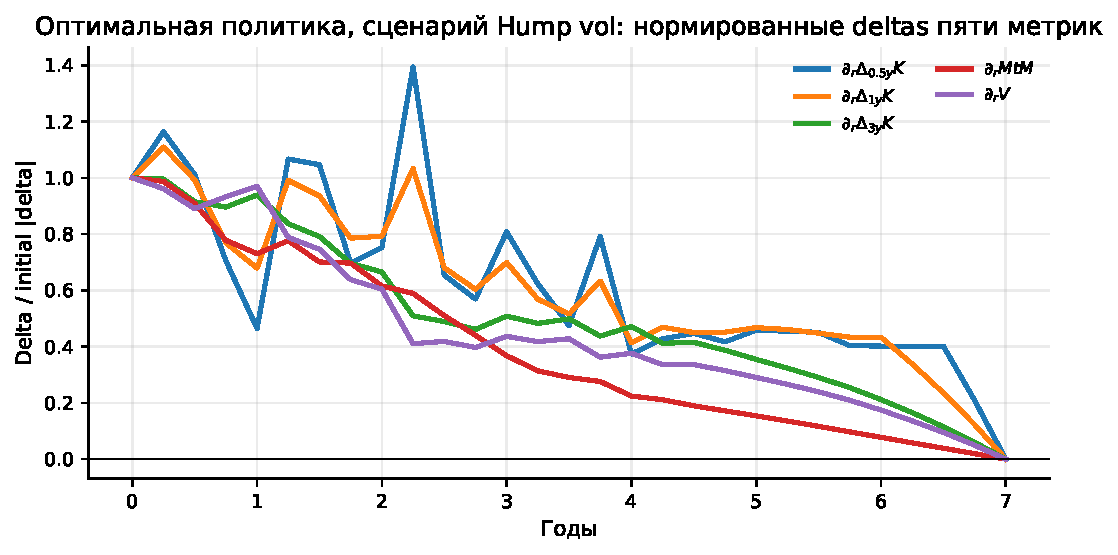
\includegraphics[width=0.93\linewidth]{figures/optimal_hump_normalized_deltas.pdf}
  \caption{Нормированные deltas пяти метрик вдоль оптимальной траектории в сценарии Hump vol. Сравнение в нормированном виде важно, потому что raw $\partial_r MtM$ на порядок больше horizon-metrics.}
\end{figure}

Содержательно здесь видно следующее.
\begin{itemize}
  \item $\partial_r MtM$ убывает почти монотонно: по мере укорачивания swap life портфель теряет duration.
  \item $\partial_r \Delta_{0.5y}K$ наиболее зубчатая: это short-horizon metric, чувствительная к ближайшему coupon carry и к локальным сдвигам $q_t$.
  \item $\partial_r \Delta_{1y}K$ и особенно $\partial_r \Delta_{3y}K$ сглаженнее: они усредняют ожидаемую mean reversion и будущую политику управления.
  \item $\partial_r V$ сидит между long-horizon capital metric и MtM: в ней одновременно видны и дальний carry, и опциональность на будущее сокращение позиции.
\end{itemize}

\subsection*{4.3. Полный retrospective atlas по сценариям и политикам}
Следующий atlas сводит вместе все $25$ комбинаций $(\text{сценарий},\text{политика})$. В каждом маленьком окне показаны нормированные траектории пяти risk-metric deltas; вертикальные штрихи соответствуют моментам $t=1y$ и $t=3y$, для которых ниже отдельно показаны state-slices.

\clearpage
\begin{landscape}
\thispagestyle{plain}
\begin{center}
  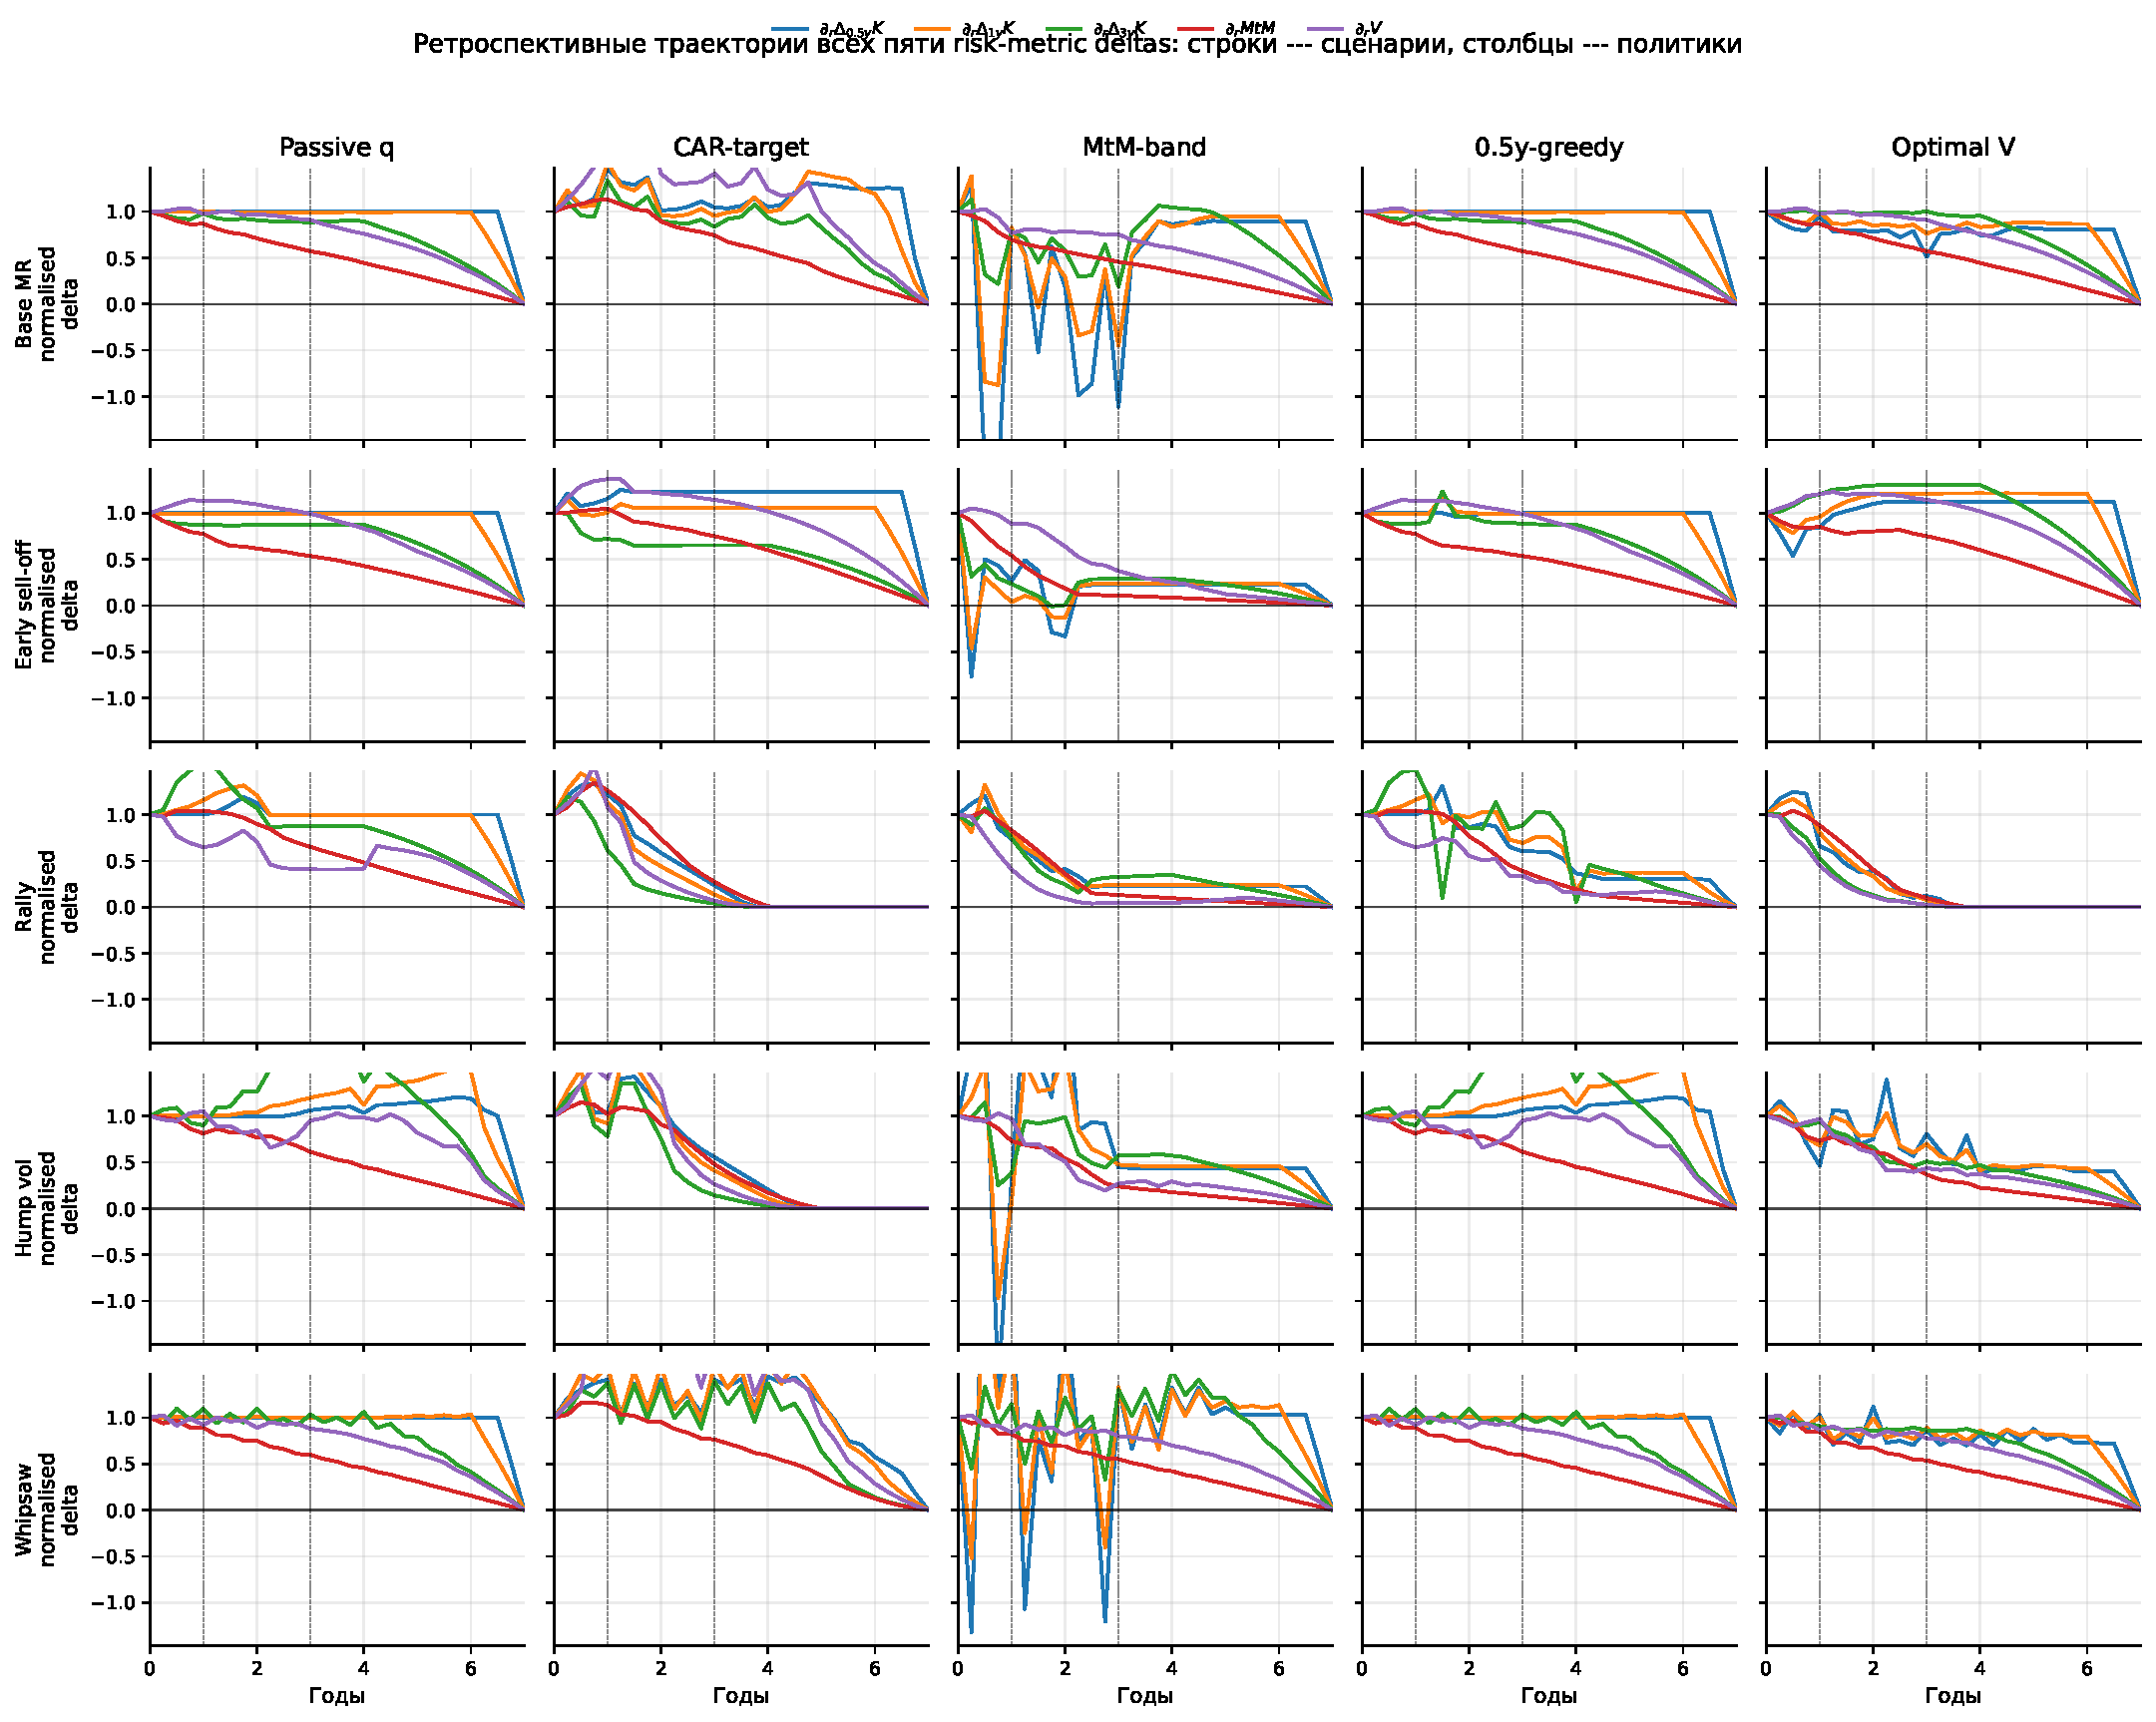
\includegraphics[width=0.95\linewidth,height=0.78\textheight,keepaspectratio]{figures/retrospective_metric_grid.pdf}

  \captionof{figure}{Ретроспективные траектории нормированных deltas всех пяти метрик. Такой формат позволяет сразу увидеть, какие сочетания сценария и политики порождают наиболее резкие перестройки rate-risk профиля.}
\end{center}
\end{landscape}
\clearpage

\subsection*{4.4. Сводка по всем сценариям и политикам}
\begin{figure}[htbp]
  \centering
  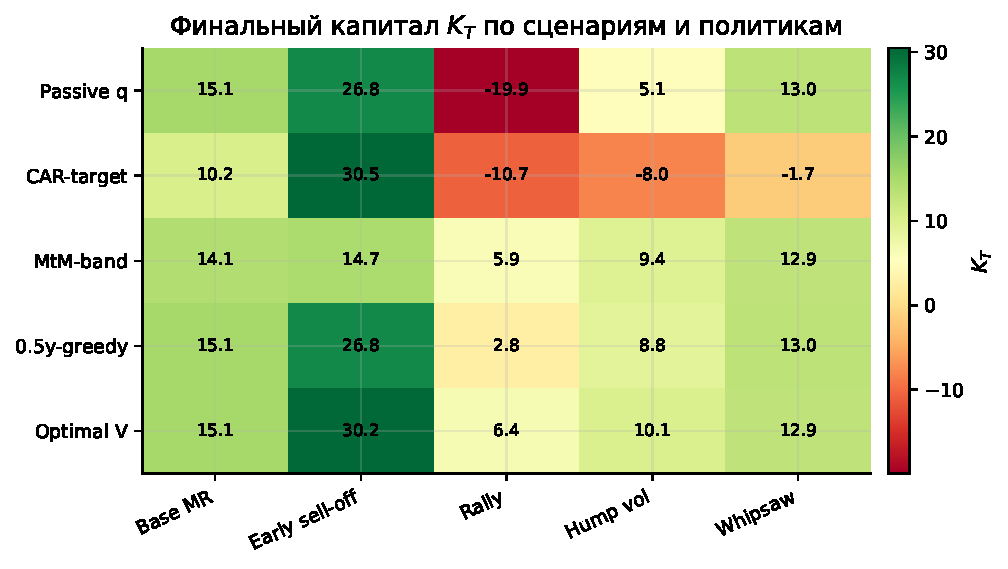
\includegraphics[width=0.92\linewidth]{figures/finalK_heatmap.pdf}
  \caption{Финальный капитал $K_T$. Полный optimal-control выигрывает в \textit{Rally} и \textit{Hump vol}, почти не уступая пассивной позиции в спокойных сценариях.}
\end{figure}

\begin{figure}[htbp]
  \centering
  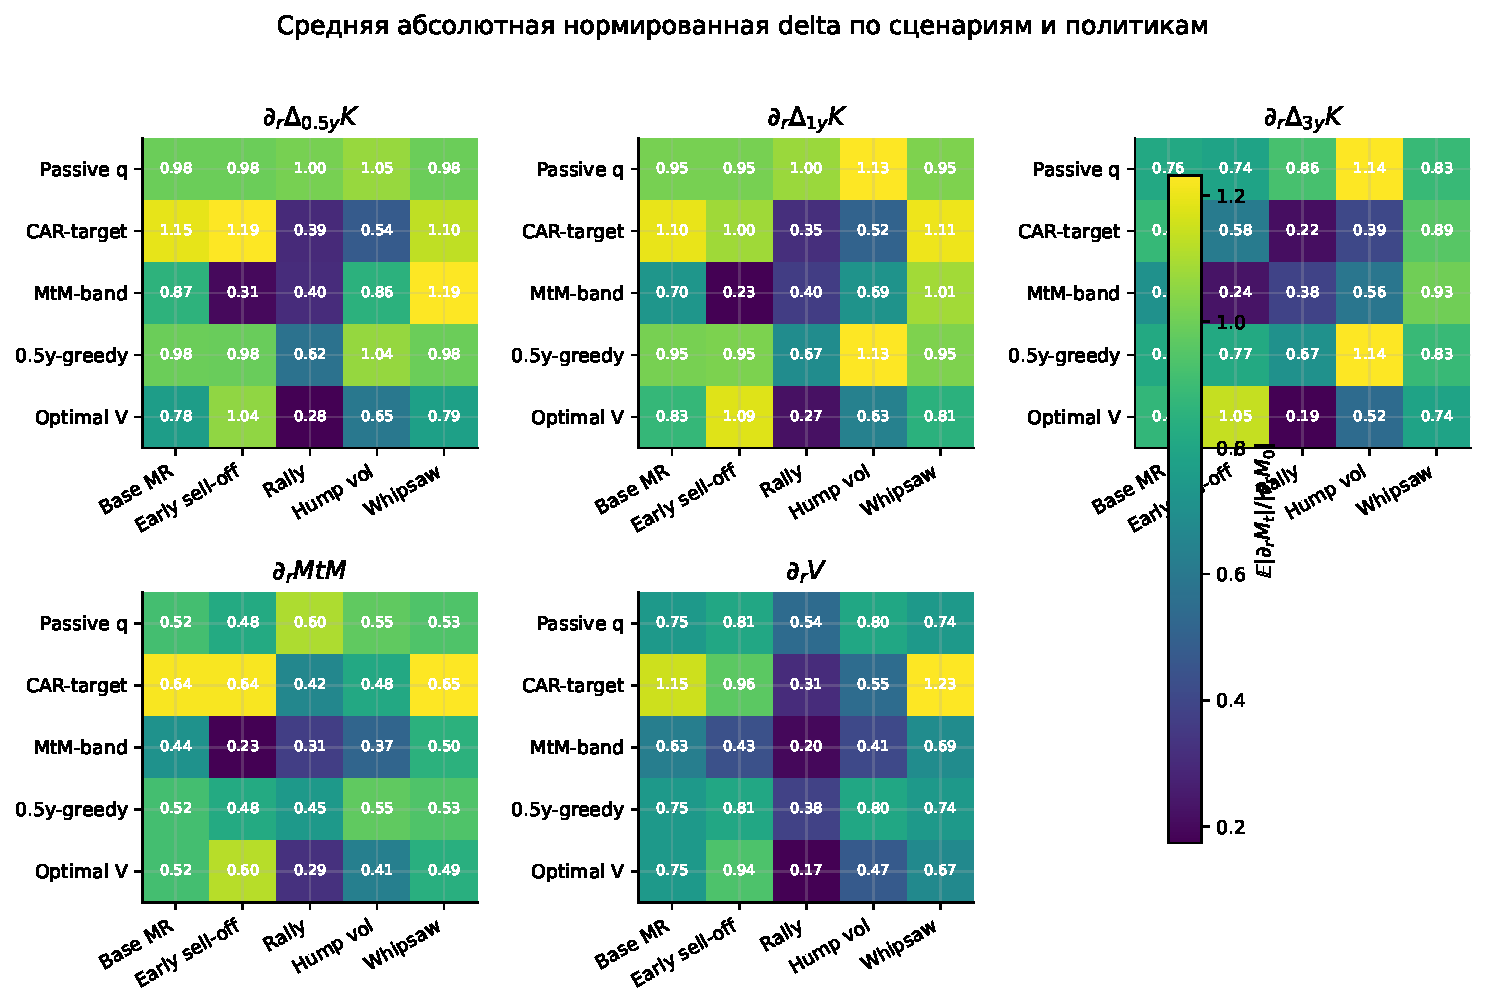
\includegraphics[width=0.97\linewidth]{figures/delta_heatmaps.pdf}
  \caption{Средняя абсолютная нормированная delta каждой из пяти метрик. Нормировка на стартовую абсолютную delta делает сценарии и политики сопоставимыми на одной шкале.}
\end{figure}

Численно финальный капитал выглядит так.

\begin{fittable}
\begin{tabular}{lrrrrr}
\toprule
Политика & Base MR & Early sell-off & Rally & Hump vol & Whipsaw \\
\midrule
Passive q & 15.13 & 26.83 & -19.93 & 5.06 & 13.02 \\
CAR-target & 10.21 & 30.46 & -10.74 & -8.00 & -1.72 \\
MtM-band & 14.13 & 14.69 & 5.91 & 9.43 & 12.86 \\
0.5y-greedy & 15.13 & 26.83 & 2.82 & 8.85 & 13.02 \\
Optimal V & 15.13 & 30.25 & 6.41 & 10.09 & 12.93 \\
\bottomrule
\end{tabular}

\end{fittable}

Две самые показательные stress-ситуации --- Rally и Hump vol --- собраны отдельно.

\begin{fittable}[\scriptsize]
\begin{tabular}{llrrrrr}
\toprule
Сценарий & Политика & Финальный K & Штраф & Ликвидность & Доля времени в breach & max |MtM| \\
\midrule
Rally & Passive q & -19.93 & 20.00 & 0.00 & 0.71 & 25.04 \\
Rally & CAR-target & -10.74 & 11.00 & 6.28 & 0.50 & 25.32 \\
Rally & MtM-band & 5.91 & 0.00 & 3.20 & 0.00 & 15.62 \\
Rally & 0.5y-greedy & 2.82 & 0.00 & 1.90 & 0.29 & 24.85 \\
Rally & Optimal V & 6.41 & 0.00 & 3.40 & 0.00 & 16.74 \\
Hump vol & Passive q & 5.06 & 4.00 & 0.00 & 0.14 & 12.22 \\
Hump vol & CAR-target & -8.00 & 13.00 & 6.42 & 0.54 & 13.22 \\
Hump vol & MtM-band & 9.43 & 0.00 & 2.38 & 0.00 & 7.38 \\
Hump vol & 0.5y-greedy & 8.85 & 0.00 & 0.30 & 0.07 & 12.22 \\
Hump vol & Optimal V & 10.09 & 0.00 & 1.00 & 0.00 & 9.16 \\
\bottomrule
\end{tabular}

\end{fittable}

\subsection*{4.5. Почему naive политики ведут себя по-разному}
\begin{figure}[htbp]
  \centering
  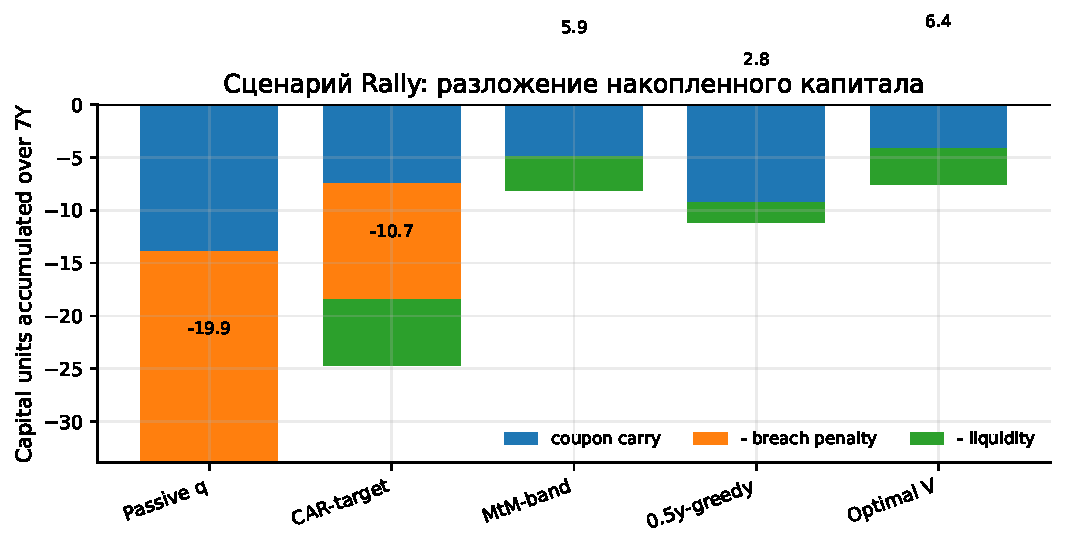
\includegraphics[width=0.92\linewidth]{figures/rally_decomposition.pdf}
  \caption{Сценарий Rally: разложение итогового капитала на coupon carry, breach penalty и liquidity cost. Пассивная позиция ловит большой отрицательный carry и штрафы; optimal и MtM-band рано сжимают номинал и тем самым режут левый хвост.}
\end{figure}

\begin{figure}[htbp]
  \centering
  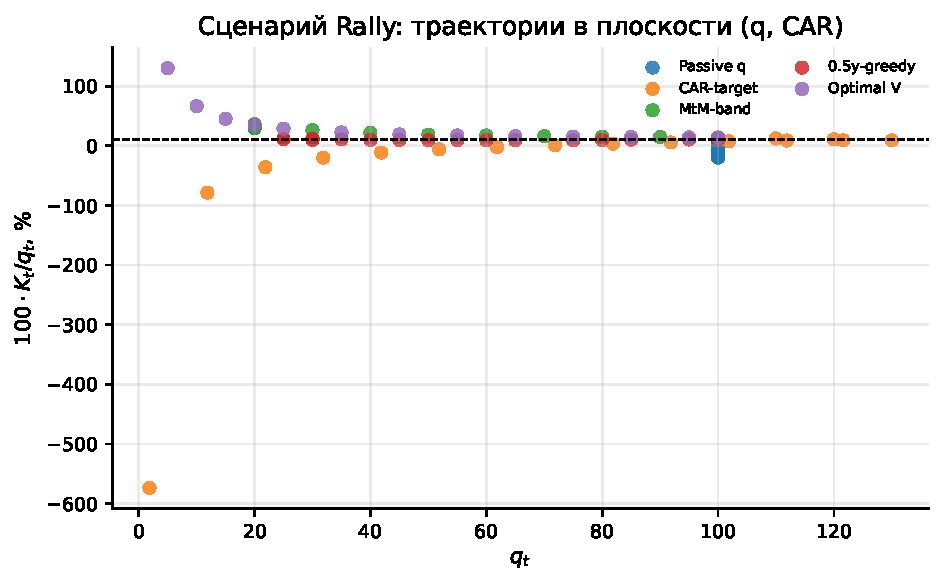
\includegraphics[width=0.82\linewidth]{figures/rally_q_car_scatter.pdf}
  \caption{Сценарий Rally в координатах $(q_t, K_t/q_t)$. CAR-target механически гонится за целевым плечом, но при ограничении на скорость не успевает вернуться в безопасную зону и накапливает штраф.}
\end{figure}

Здесь главный qualitative takeaway такой:
\begin{itemize}
  \item \textbf{Passive q} сохраняет upside в sell-off, но берет на себя весь downside в rally.
  \item \textbf{CAR-target} интуитивен, но слишком локален: когда капитал уже просел, ограничения на скорость и liquidity cost не дают быстро восстановить отношение $K/q$.
  \item \textbf{MtM-band} хорошо стабилизирует рыночную стоимость и почти всегда держит CAR выше порога, но часто преждевременно отрезает profitable exposure.
  \item \textbf{0.5y-greedy} полезна в коротком stress-window, но систематически недооценивает дальний эффект будущих штрафов.
  \item \textbf{Optimal V} лучше всего балансирует carry, future deleveraging option и penalty avoidance. Именно поэтому она доминирует в Rally и чуть лучше других защитных правил в Hump vol.
\end{itemize}

\subsection*{4.6. Геометрия оптимального контроля}
\begin{figure}[htbp]
  \centering
  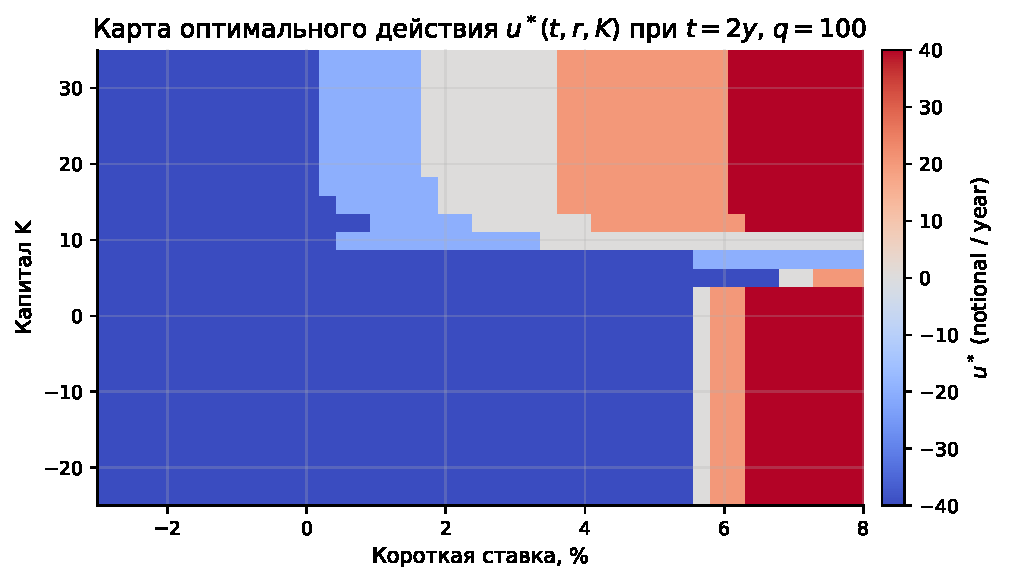
\includegraphics[width=0.88\linewidth]{figures/optimal_policy_map.pdf}
  \caption{Срез оптимального правила управления при $t=2y$ и $q=100$. Низкий капитал и низкая ставка толкают к отрицательному $u^*$ (де-рискинг); высокий капитал и высокий short rate позволяют удерживать или даже наращивать номинал.}
\end{figure}

\section*{5. Зависимость risk-metrics от состояния агента}
Чтобы увидеть, как метрики зависят именно от состояния $s=(r,q,K)$, ниже зафиксированы координатные срезы по reference path \textit{Base MR + Optimal V}: в моменты $t=0$, $1y$ и $3y$ две координаты держатся на reference-state, а третья варьируется по сетке. Для horizon-capital метрик показаны все пять политик; для $MtM$ и $V$ линия одна, потому что при фиксированном состоянии это policy-invariant объекты.

\clearpage
\begin{landscape}
\thispagestyle{plain}
\begin{center}
  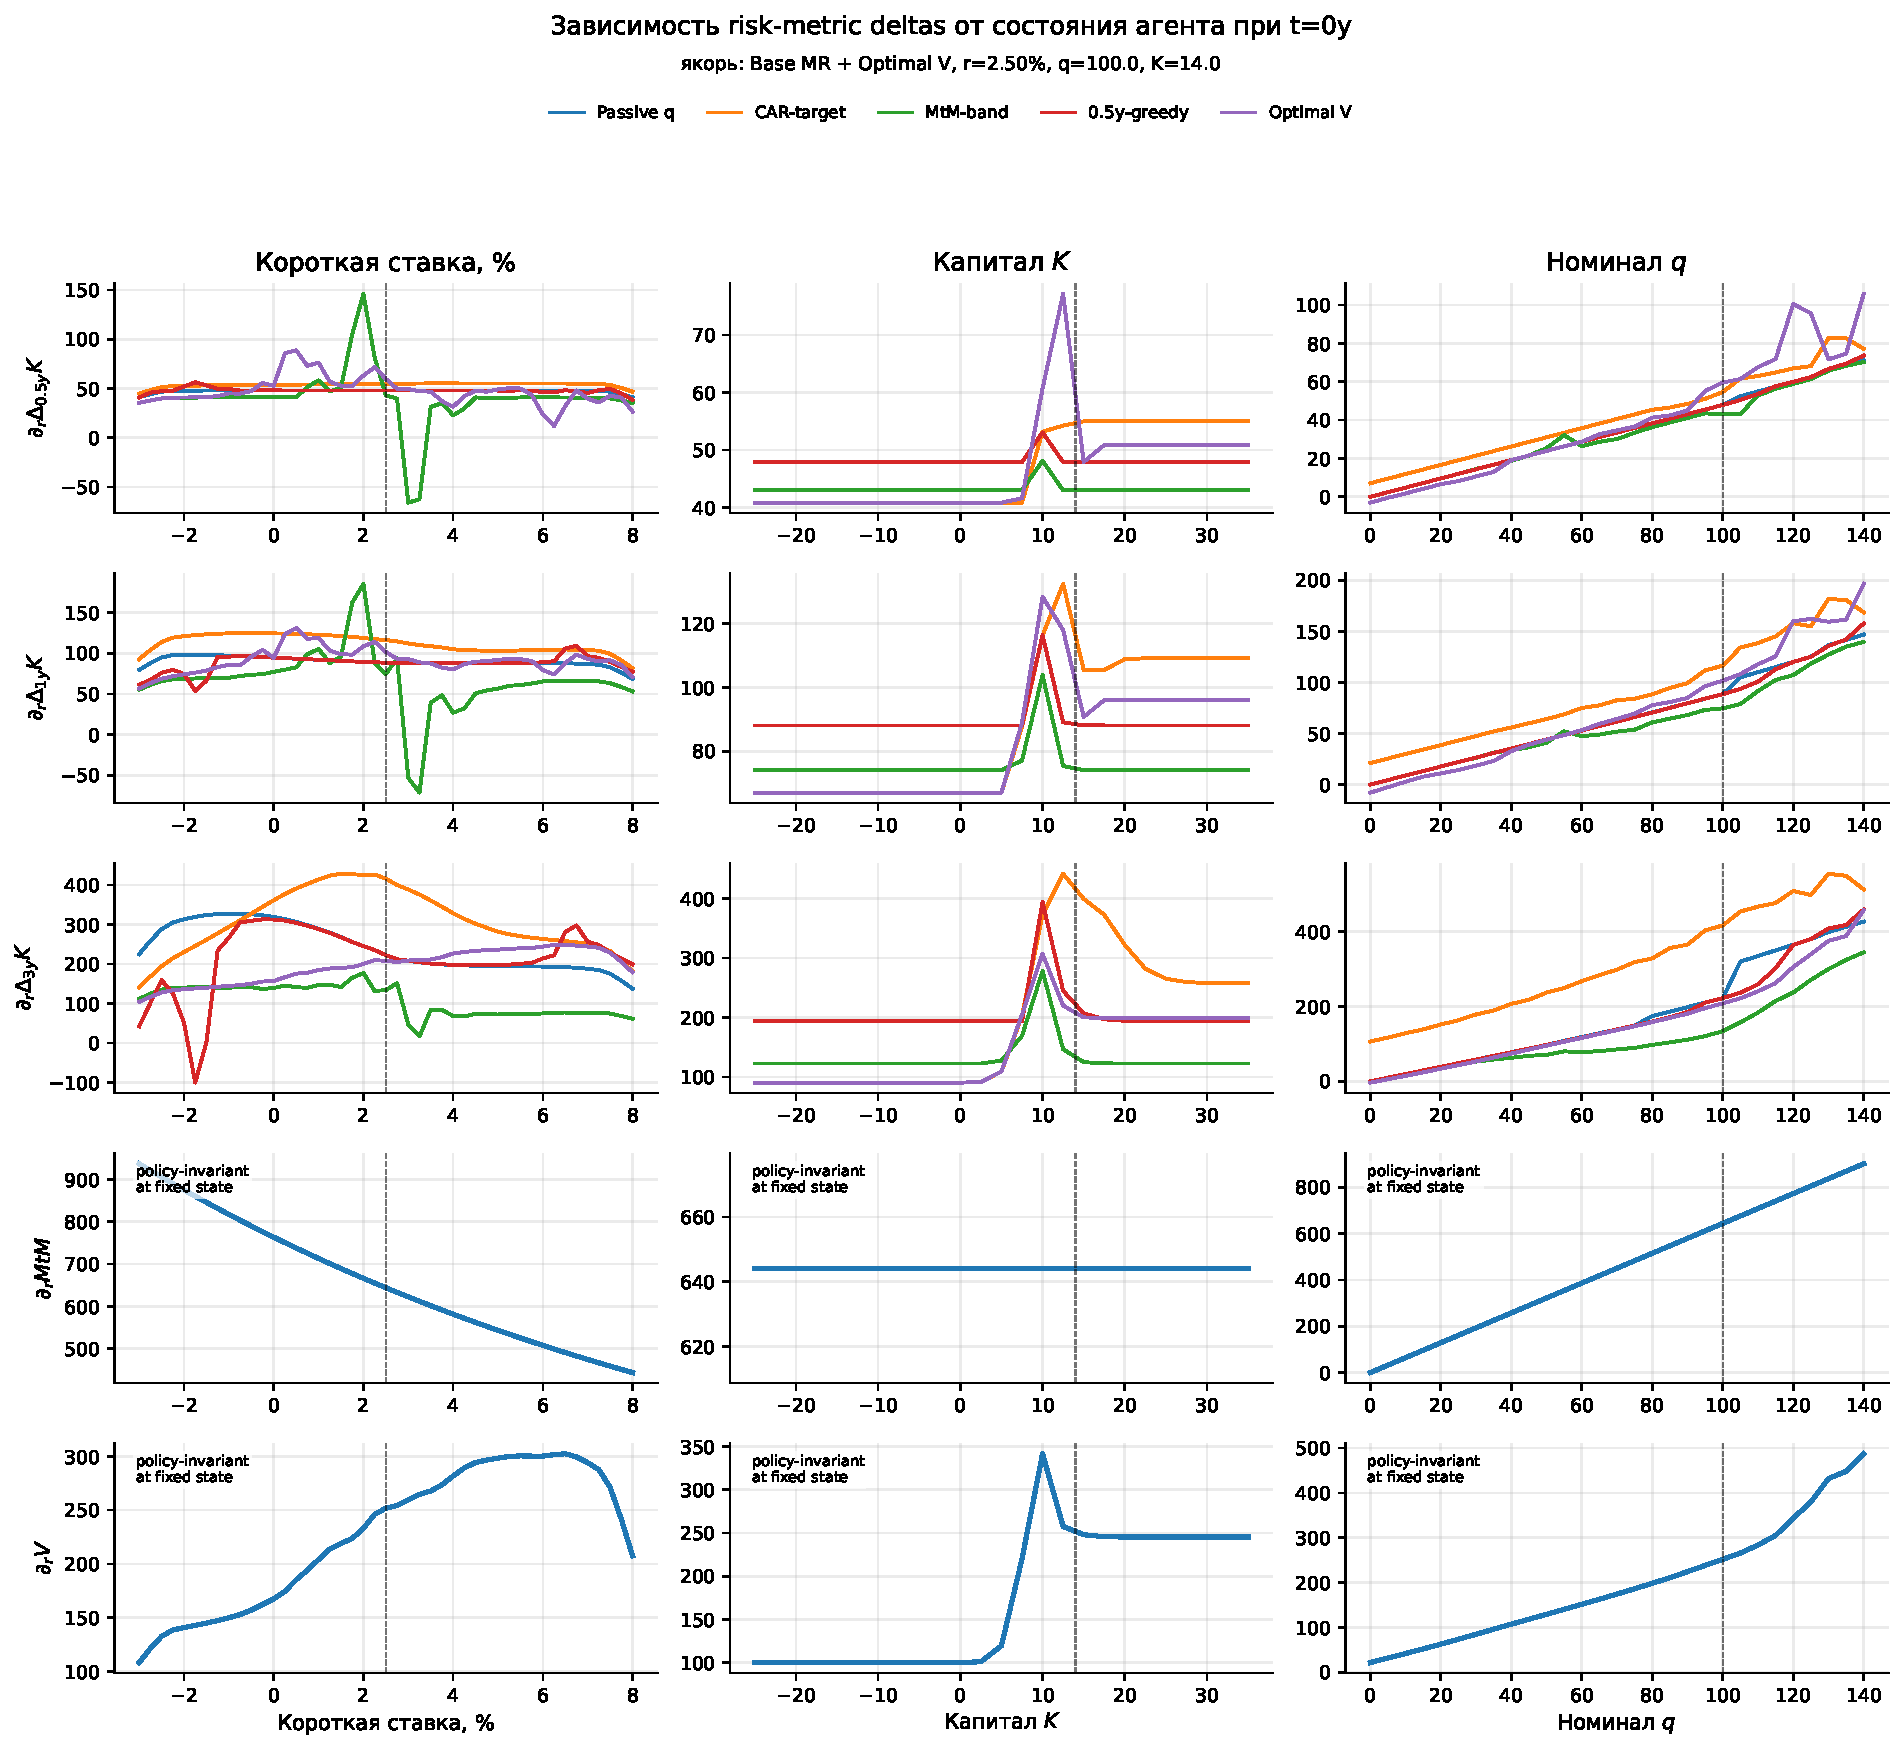
\includegraphics[width=0.95\linewidth,height=0.80\textheight,keepaspectratio]{figures/state_slices_t0p0.pdf}

  \captionof{figure}{State-slices risk-metric deltas в начальном состоянии $t=0$. Штриховая вертикаль отмечает reference-state $(r_0,q_0,K_0)$.}
\end{center}
\end{landscape}
\clearpage

\clearpage
\begin{landscape}
\thispagestyle{plain}
\begin{center}
  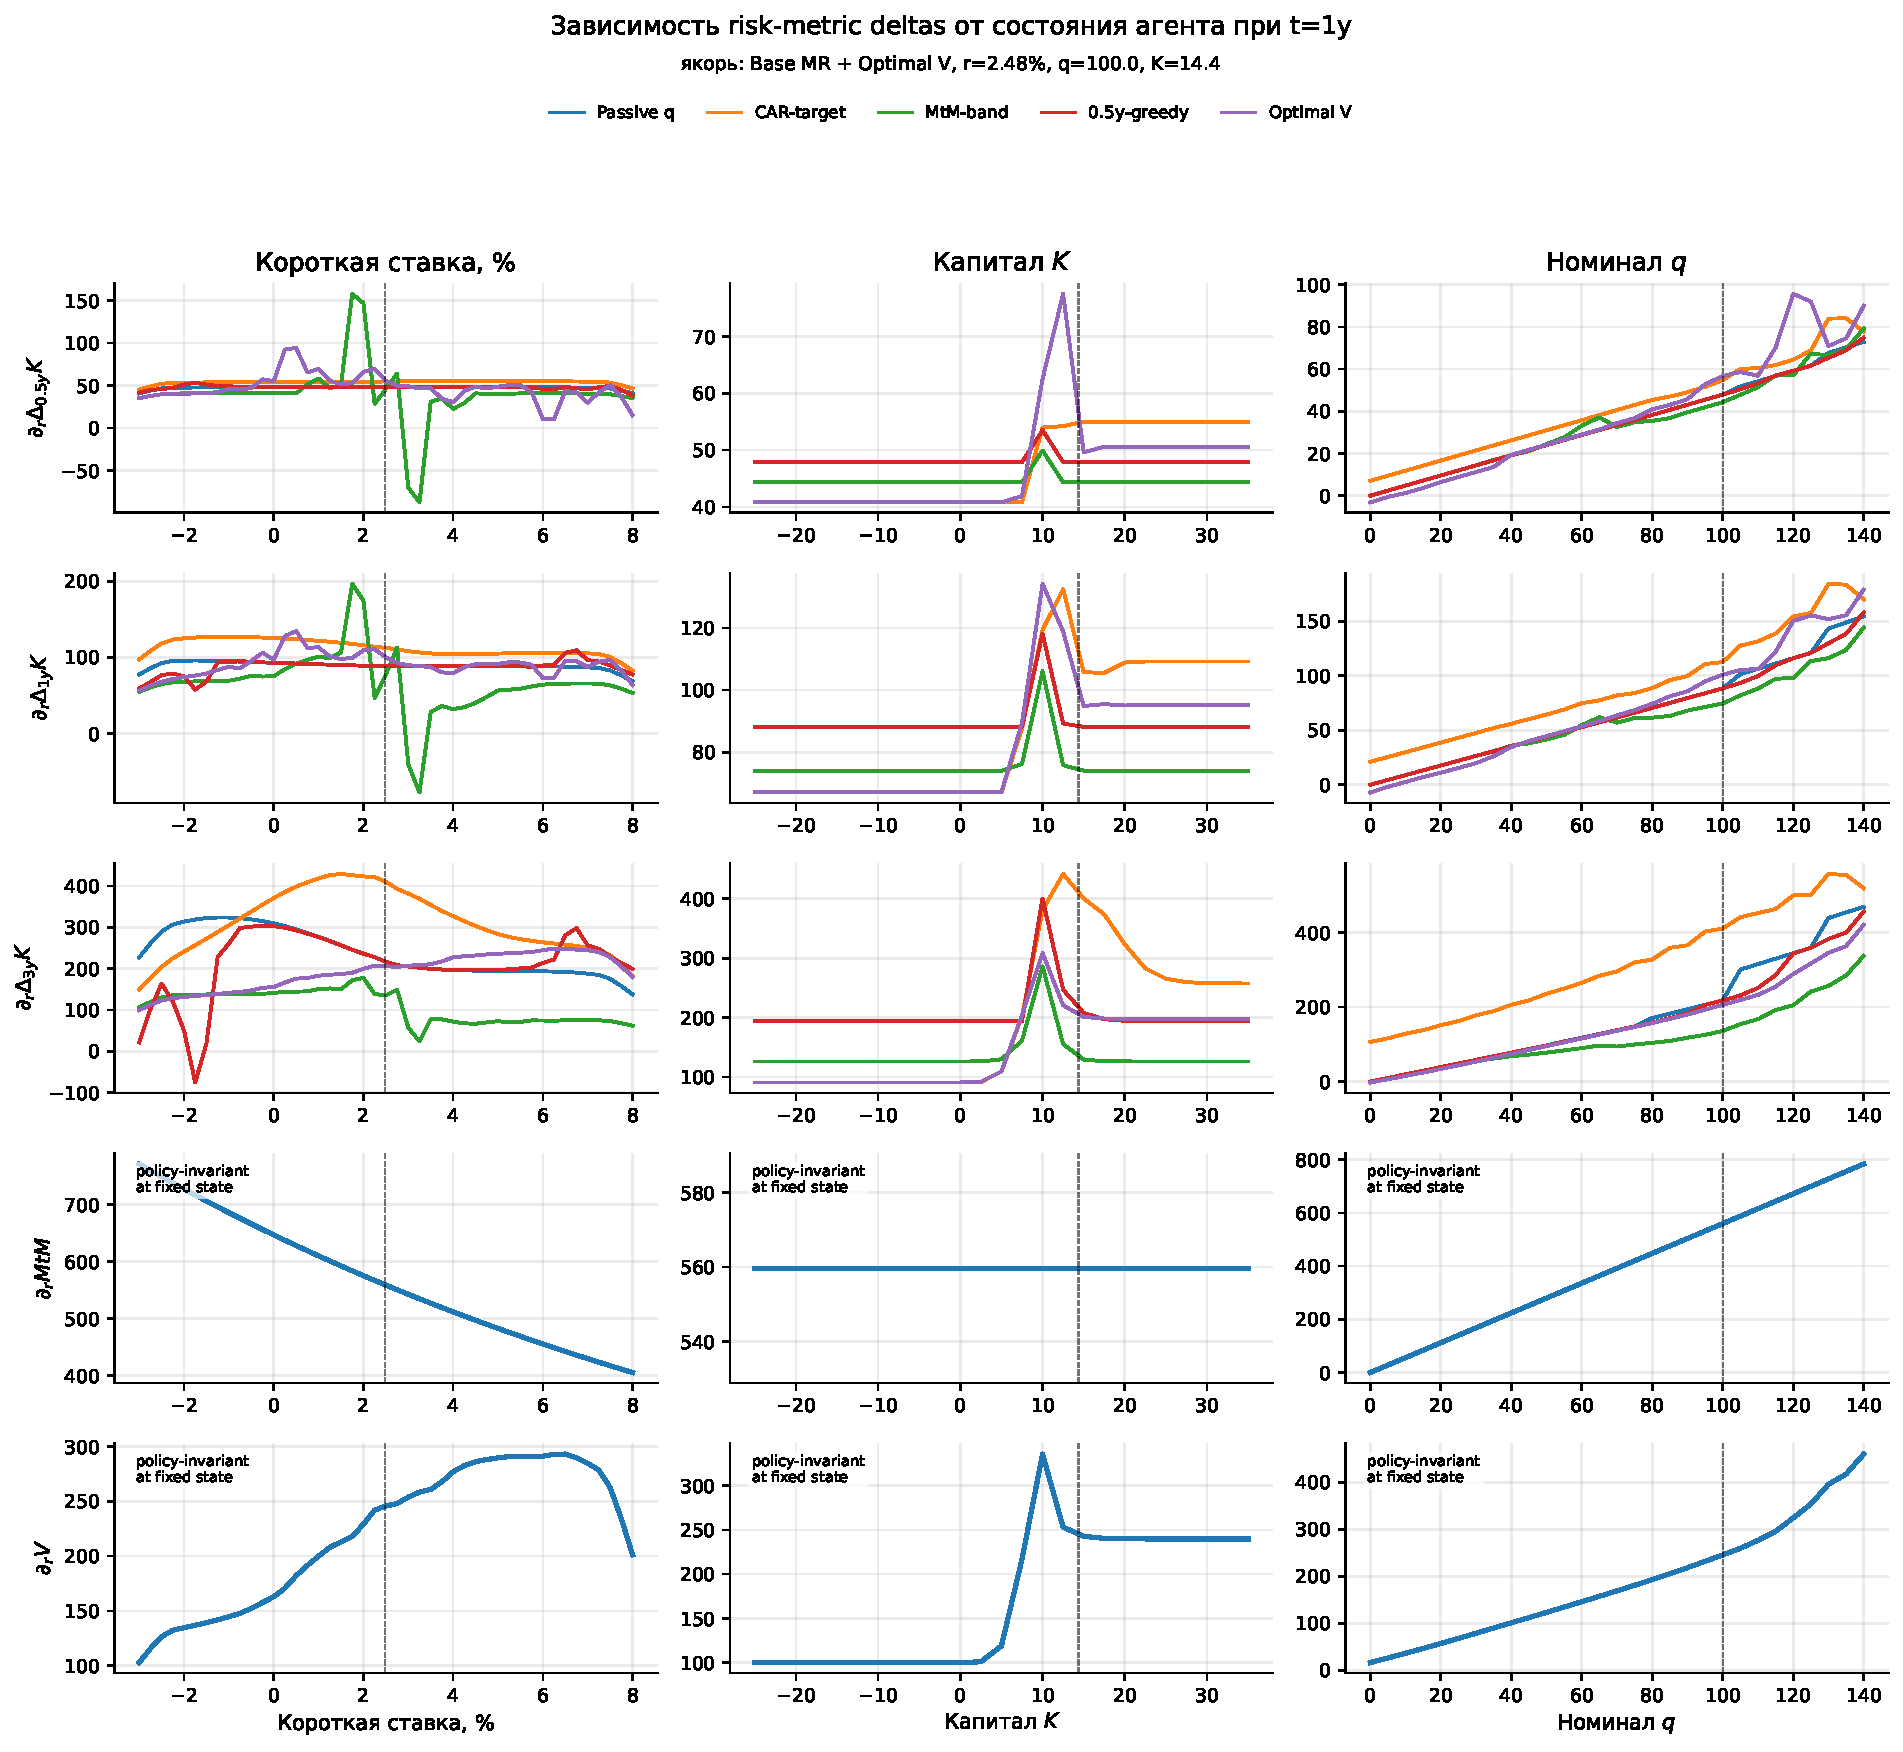
\includegraphics[width=0.95\linewidth,height=0.80\textheight,keepaspectratio]{figures/state_slices_t1p0.pdf}

  \captionof{figure}{State-slices через $1$ год. Видно, что чувствительность horizon-capital метрик к $K$ и $q$ становится более нелинейной, особенно рядом с областью $K/q \approx CAR$.}
\end{center}
\end{landscape}
\clearpage

\clearpage
\begin{landscape}
\thispagestyle{plain}
\begin{center}
  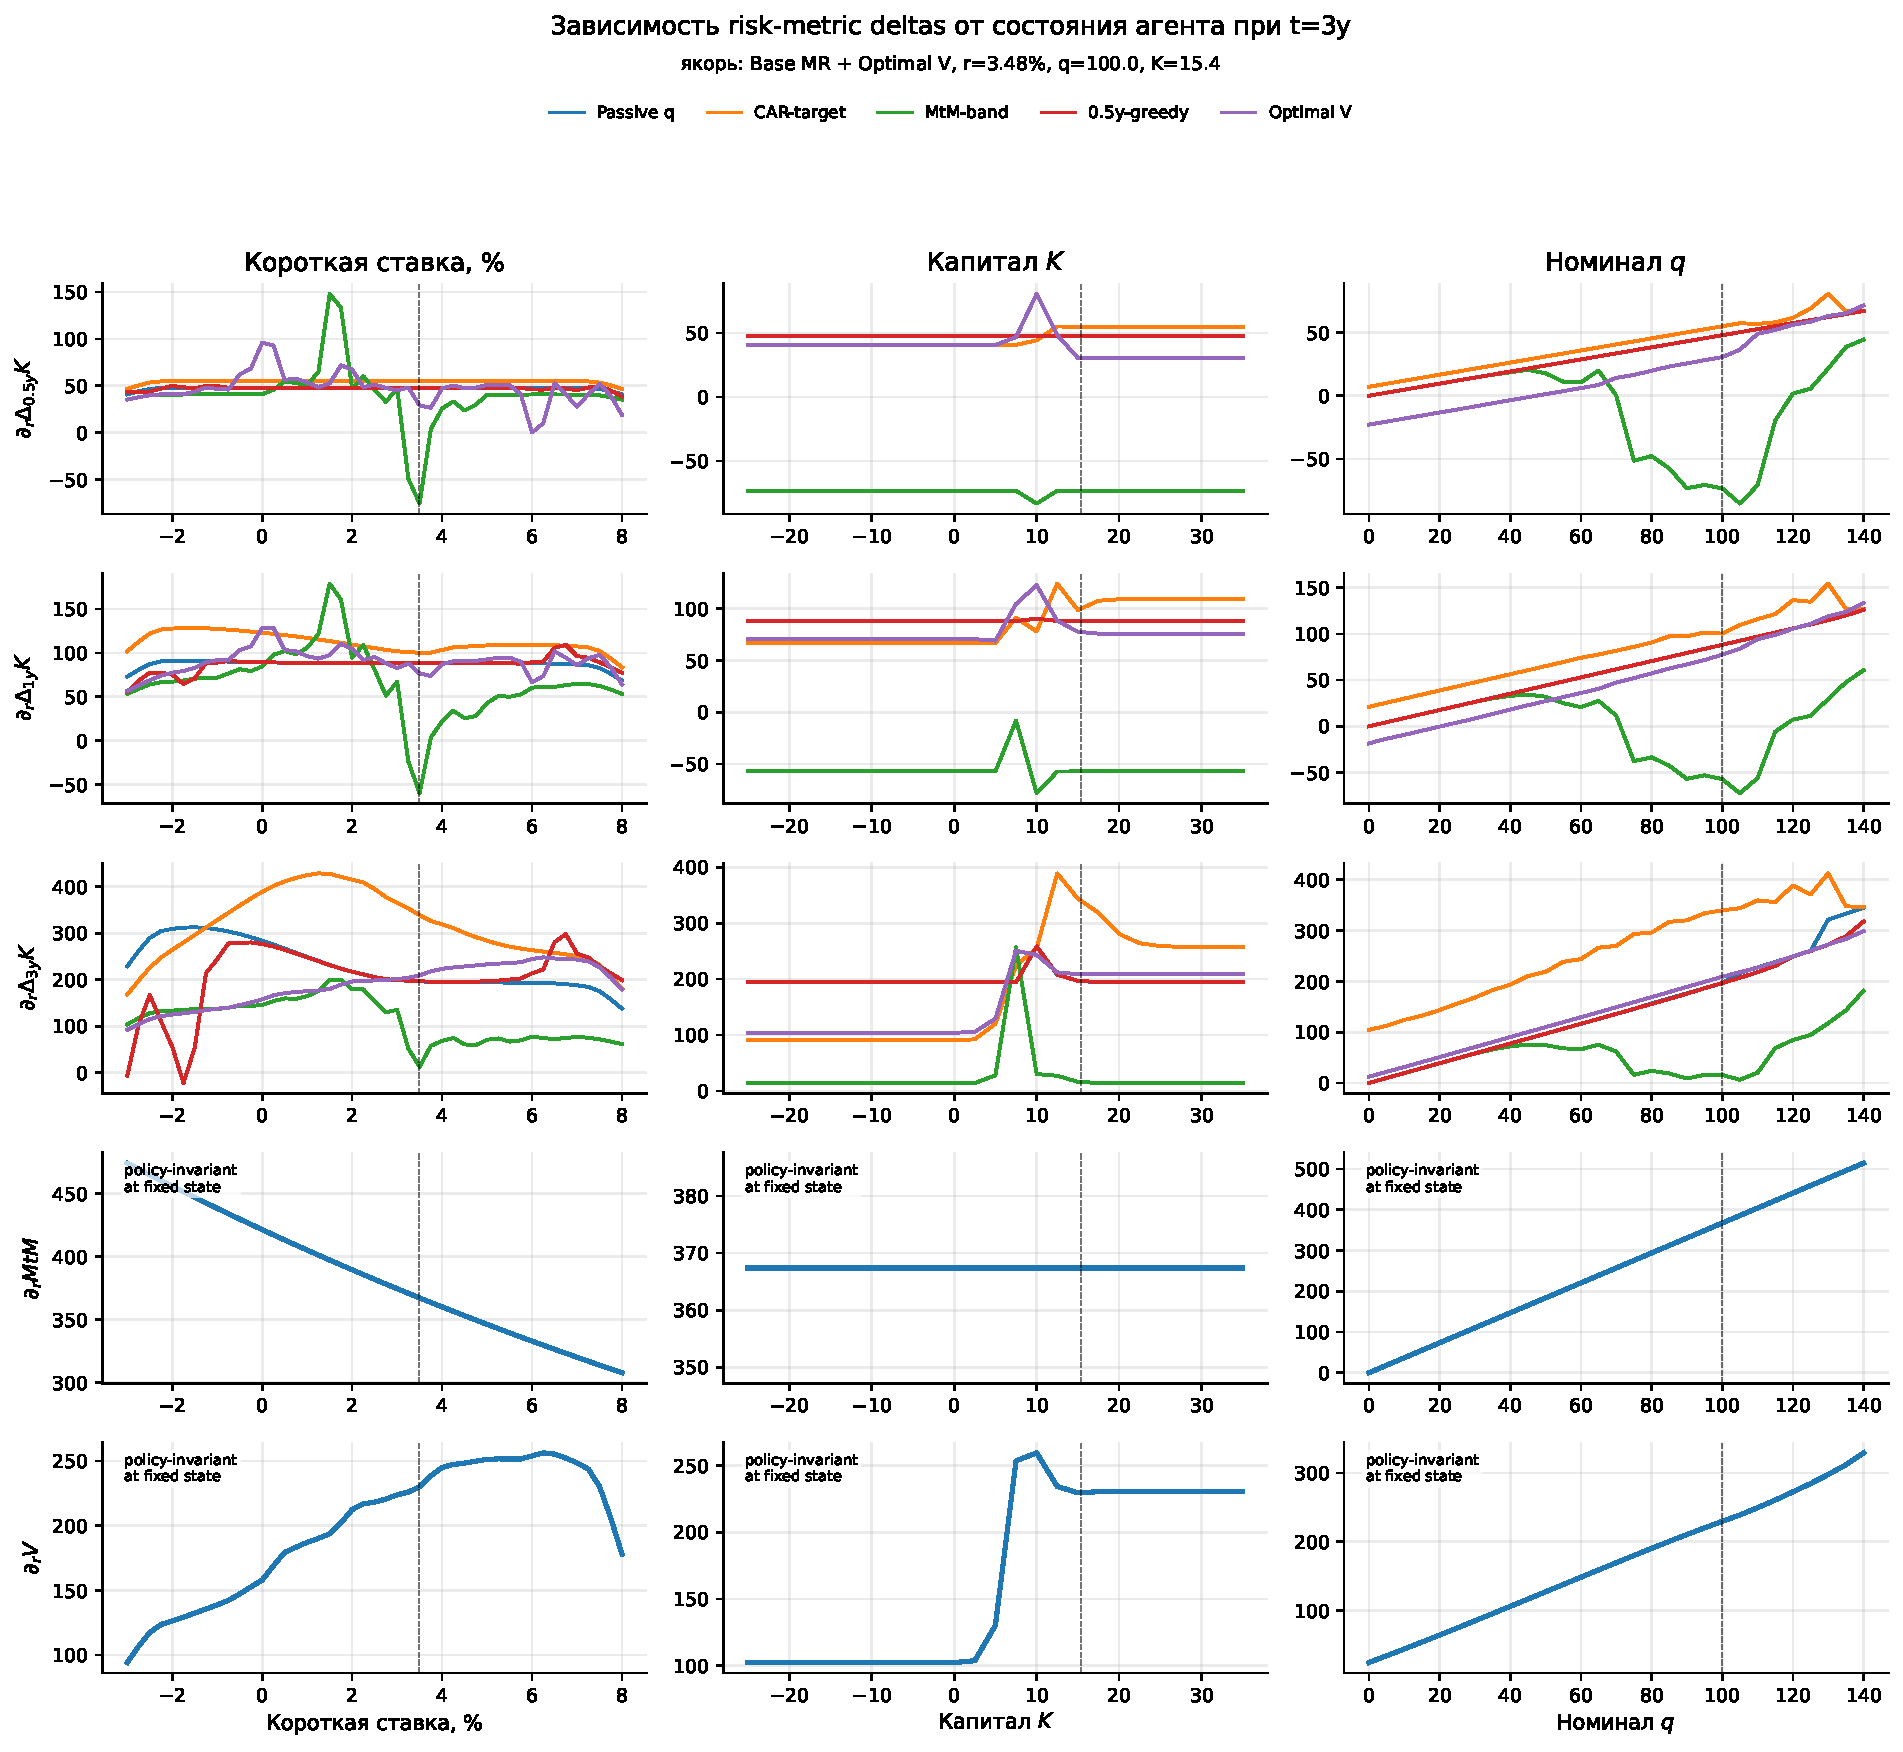
\includegraphics[width=0.95\linewidth,height=0.80\textheight,keepaspectratio]{figures/state_slices_t3p0.pdf}

  \captionof{figure}{State-slices через $3$ года. По мере укорачивания свопа рынок теряет duration, а управленческие метрики сильнее отражают оставшуюся опциональность на deleveraging.}
\end{center}
\end{landscape}
\clearpage

Из этих state-slices удобно читать три общих эффекта.
\begin{itemize}
  \item При снижении $r$ horizon-capital deltas быстро становятся более отрицательными для правил, которые aggressively режут $q_t$: desk заранее страхуется от будущего отрицательного carry и от риска попасть в breach-zone.
  \item Чувствительность по $K$ имеет kink около границы $K/q \approx CAR$: это прямой след штрафа за нахождение в forbidden-zone и ограничения на скорость изменения позиции.
  \item Зависимость по $q$ сильнее всего различает политики: passive и short-horizon greedy почти линейны, тогда как CAR-target и full-optimal сильнее сглаживают хвосты за счёт будущего deleveraging.
\end{itemize}

\subsection*{5.1. Интерпретация пяти rate-risk метрик}
Если смотреть именно на retrospective поведение deltas и их state-slices, то toy-example показывает вполне характерную картину.
\begin{enumerate}[label=\arabic*)]
  \item \textbf{$\partial_r MtM$} --- самая "рынковая" метрика: она почти не зависит от capital friction напрямую и потому сильнее всего отражает остаточную duration позиции.
  \item \textbf{$\partial_r \Delta_{0.5y}K$} --- наиболее близка к carry/risk-budget операционному управлению на горизонте ALM desk.
  \item \textbf{$\partial_r \Delta_{1y}K$} и \textbf{$\partial_r \Delta_{3y}K$} уже чувствуют структуру будущих решений по $q_t$, так что это не просто "swap delta", а delta контролируемой капитальной траектории.
  \item \textbf{$\partial_r V$} --- наиболее содержательная управленческая delta: в ней собран и carry, и риск breach-зоны, и цена ограниченной ликвидности.
  \item Ни одна из метрик не является "лучшей" сама по себе. Выбор зависит от того, что desk действительно минимизирует: мгновенный MtM risk, ближайший capital carry, либо full-horizon franchise value.
\end{enumerate}


\section*{6. Проверка расчётов и воспроизводимость}
После повторного прогона расчётов были сделаны несколько независимых численных проверок.
\begin{itemize}
  \item аналитическая формула для $\partial_r MtM$ сверена с центральной конечной разностью;
  \item на всех $25$ траекториях проверена тождественность $K_T = K_0 + \sum_t \Delta K_t$;
  \item отдельно проверено разложение $\Delta K_t = \text{coupon} - \text{penalty} - \text{liquidity}$;
  \item summary-таблицы и CSV пересчитаны из симулированных путей и совпали до машинной точности;
  \item на случайной выборке узлов сетки проверено уравнение Беллмана для $V_t$ и совпадение сохранённой оптимальной политики с повторным $\arg\max$.
\end{itemize}

\begin{fittable}
\begin{tabular}{lllll}
\toprule
Check & Max abs error & Mean abs error & Tolerance & Pass \\
\midrule
swap delta finite-difference & 6.42e-09 & 2.37e-09 & 1.0e-06 & yes \\
capital path recursion & 1.07e-14 & 3.82e-15 & 1.0e-10 & yes \\
dK decomposition & 7.11e-15 & 7.13e-16 & 1.0e-10 & yes \\
summary CSV consistency & 0.00e+00 & 0.00e+00 & 1.0e-12 & yes \\
Bellman residual on sampled states & 3.55e-15 & 9.59e-17 & 1.0e-08 & yes \\
Optimal action matches stored policy & 0.00e+00 & 0.00e+00 & 0.0e+00 & yes \\
MtM start delta formula & 0.00e+00 & 0.00e+00 & 1.0e-12 & yes \\
\bottomrule
\end{tabular}

\end{fittable}

Практически это означает, что повторный прогон дал те же summary-результаты, что и в предыдущей версии артефактов: различия по всем числовым полям не превышают машинного округления порядка $10^{-14}$--$10^{-16}$.

\section*{7. Что важно помнить}

Это \textbf{toy-example}, а не production pricing / XVA / ALM engine. В частности:
\begin{itemize}
  \item использован один фактор Hull-White и flat-curve proxy для MtM;
  \item параметры под real-world и pricing measure взяты одинаковыми;
  \item управление ограничено простым дискретным набором скоростей;
  \item штраф breach-зоны задан намеренно жестко, чтобы поведение политик было видно на графиках.
\end{itemize}
Но даже в таком упрощенном сетапе хорошо видно главное: \textbf{метрика риска определяет не только то, как мы измеряем позицию, но и то, как именно будет выглядеть оптимальное управление номиналом.}

{\small Базовые ориентиры по модели: Hull \& White (1990), Brigo \& Mercurio (2006).}

\end{document}
